% Build with custom engines, which move all miscellaneous files into a 'build' folder.
% See https://tex.stackexchange.com/questions/67211/use-texshop-preview-window-when-different-output-dir-is-set

%% ------ Packages ------ %%
% Related to the document setup:
\documentclass[12pt, a4paper]{extarticle}
\usepackage[a4paper, top = 2.4cm, bottom = 2.4 cm, right= 2.1cm, left= 2.1cm]{geometry}
\usepackage[english]{babel}
\renewcommand\familydefault{\sfdefault}
\usepackage{amsmath}
\usepackage{mathtools}
\usepackage{amsfonts}
\usepackage{amssymb}

\usepackage[T1]{fontenc}
\setlength\parindent{0pt}
\usepackage{multicol}
\usepackage{xspace}


% Colouring the references
\usepackage{hyperref}
\usepackage{cleveref}
\usepackage[dvipsnames]{xcolor}
\pagecolor{white}
\newcommand\myshade{85}
\colorlet{mylinkcolor}{violet}
\colorlet{mycitecolor}{YellowOrange}
\definecolor{myurlcolor}{rgb}{ 0, 0.4470, 0.6410}

\hypersetup{
  linkcolor  = mylinkcolor!\myshade!black,
  citecolor  = mycitecolor!\myshade!black,
  urlcolor   = myurlcolor!\myshade!black,
  colorlinks = true,
}

% Nomenclature
%\usepackage{nomencl}
%\makenomenclature
%%\renewcommand{\nomname}{List of symbols}
%\renewcommand{\nompreamble}{\noindent Definitions of the nomenclature}
%\newlength{\nomitemorigsep}
%\setlength{\nomitemorigsep}{\nomitemsep}
%\setlength{\nomitemsep}{-\itemsep}

% Section properties redefinitions
\makeatletter
\renewcommand\section{\@startsection {section}{1}{\z@}{3ex }{0.1ex } {\normalfont\large\bfseries}}
\renewcommand\subsection{\@startsection{subsection}{1}{\z@}{2ex }{0.1ex } {\normalfont \bfseries}}
\renewcommand\subsubsection{\@startsection{subsubsection}{3}{\z@}{-1.5ex\@plus -1ex \@minus -.2ex}{.5ex}{\normalfont}}
\makeatother

% Graphics interfaces:
\usepackage{graphicx}
\usepackage{tikz}
\tikzset{every picture/.style={line width=1pt}}
\usepackage{float}
\usepackage{subcaption} 
\usepackage[font=small,aboveskip=3pt, belowskip=-0pt]{caption}


% Headers and footers:
\usepackage{url}
\usepackage{footnote}
\usepackage{fancyhdr}
\pagestyle{fancy} 
\fancyhf{} 
\renewcommand{\headrulewidth}{0pt}
\newcommand{\mainmatter}{\clearpage \cfoot{\thepage\ of \pageref{LastPage}}
\setcounter{page}{1}
\pagenumbering{arabic}}
\usepackage{comment}

% Sort the bibliography
\usepackage[sort]{cite}
\setlength\columnsep{15pt}

% Command definitions:
\newcommand{\dtheta}{{\dot{\theta}}\xspace}
\newcommand{\ic}{{\rm{i}}\xspace}

\renewcommand{\Re}{{\operatorname{Re}}\xspace}
\newcommand{\R}{{\rm I\!R}\xspace}
\newcommand{\C}{{\mathbb{C}}\xspace}
\newcommand{\T}{{\mathbb{T}}\xspace}

\renewcommand{\k}{{\boldsymbol{k}}\xspace}
\newcommand{\kacc}{{\boldsymbol{k'}}\xspace}
\newcommand{\kmean}{{\langle k\rangle}\xspace}
\newcommand{\kin}{{k^{\rm in}}\xspace}
\newcommand{\kout}{{k^{\rm out}}\xspace}
\newcommand{\degree}{{\rm deg}\xspace}

\newcommand{\tp}{{t^{\prime}}\xspace}
\newcommand{\tpp}{{t^{\prime \prime}}\xspace}

\newcommand{\Sin}{{S^{\rm in}}\xspace}
\newcommand{\Sout}{{S^{\rm out}}\xspace}

\newcommand{\mfr}{{\textsl{MFR}}\xspace}
\newcommand{\SNIC}{{\textsl{SNIC}}\xspace}
\newcommand{\PSR}{{\textsl{PSR}}\xspace}
\newcommand{\PSS}{{\textsl{PSS}}\xspace}
\newcommand{\CPW}{{\textsl{CPW}}\xspace}
\newcommand{\STDP}{{\textsl{STDP}}\xspace}
\newcommand{\LTP}{{LTP}\xspace}
\newcommand{\LTD}{{LTD}\xspace}

\def\matlab{\textsc{Matlab}\xspace}


%% ------ Front page ------ %%

\begin{document}

\mainmatter

\pagenumbering{Roman}
% !TEX root = ../main.tex

\begin{titlepage} % Suppresses displaying the page number on the title page and the subsequent page counts as page 1
	\newcommand{\HRule}{\rule{\linewidth}{0.5mm}} % Defines a new command for horizontal lines, change thickness here
	
	%\center % Centre everything on the page
	
	%------------------------------------------------
	%	Headings
	%------------------------------------------------
	\begin{minipage}{\linewidth}
   	\begin{flushright}
	Msc thesis\\ Mathematical Modelling and Computation
    	\end{flushright}
 	\end{minipage}
	
	\begin{center} \begin{minipage}{0.87\linewidth}
	\begin{tikzpicture}[remember picture,overlay]
    		\node[anchor=south west,yshift=64pt,xshift=55pt]%
        		at (current page.south west)
        		{\includegraphics[height=14mm]{../Figures/Logos/ComputeLogo.png}};
	\end{tikzpicture}
	\begin{tikzpicture}[remember picture,overlay]
    		\node[anchor=south east,yshift=64pt,xshift=-55pt]%
        		at (current page.south east)
        		{\includegraphics[height=14mm]{../Figures/Logos/DTUlogoRed.png}};
	\end{tikzpicture}

	\end{minipage} \end{center}
	\vspace{100mm}
	
	
	%{\Large \department}\\[1.5cm] % Main heading such as the name of your university/college
	
	%{\large \departmentdescriber}\\[0.5cm] % Major heading such as course name
		
	%------------------------------------------------
	%	Title
	%------------------------------------------------
	
	%\HRule\\[0.4cm]
	
	{\Huge \thesistitle: \\ \thesissubtitle}\\% Title of your document
	
	%\HRule\\[1.5cm]
	
	%------------------------------------------------
	%	Author(s)
	%------------------------------------------------
	
	\begin{minipage}{0.5\textwidth}
		\begin{flushleft}
			\large
			\thesisauthor, \studentnumber
		\end{flushleft}
	\end{minipage} \\[15mm]
	\begin{minipage}{0.5\textwidth}
		\begin{flushleft}
			\large
			\textit{Supervisors}\\
			\thesissupervisorI \\
			\thesissupervisorII % Supervisor's name
		\end{flushleft}
	\end{minipage}
	
	% If you don't want a supervisor, uncomment the two lines below and comment the code above
	%{\large\textit{Author}}\\
	%John \textsc{Smith} % Your name
	
	%------------------------------------------------
	%	Date
	%------------------------------------------------
	
	\vfill\vfill % Position the date 3/4 down the remaining page
	
	{\large\thedate} % Date, change the \today to a set date if you want to be precise
	
	%------------------------------------------------
	%	Logo
	%------------------------------------------------
	
	%\vfill\vfill
	%\includegraphics[width=0.2\textwidth]{placeholder.jpg}\\[1cm] % Include a department/university logo - this will require the graphicx package
	 
	%----------------------------------------------------------------------------------------
	
	\vfill % Push the date up 1/4 of the remaining page
	
\end{titlepage}

\tableofcontents

\section*{Abstract}
\addcontentsline{toc}{subsection}{Abstract}
The synchronisation of networks of oscillators, network topology and network plasticity can only be understood from a holistic approach, and each domain is investigated in relation to the other. The Theta neuron model is analysed to understand feedback mechanisms between the frequency and phase response through the electrical current. Different network topologies are then described in terms of their degree distribution. Networks of Theta neurons are studied using the synchronisation of the mean-field. Inspired by the process of synaptic plasticity, learning rules are then established to observe emergent network topologies. 

%\section*{Acknowledgements}
%\addcontentsline{toc}{subsection}{Acknowledgements}
%thankyou thankyou thankyou thankyou thankyou thankyou thankyou thankyou thankyou thankyou thankyou thankyou thankyou thankyou thankyou thankyou thankyou thankyou thankyou thankyou thankyou thankyou thankyou thankyou thankyou thankyou thankyou thankyou thankyou thankyou thankyou thankyou thankyou thankyou thankyou thankyou thankyou thankyou thankyou thankyou thankyou thankyou thankyou thankyou thankyou thankyou thankyou thankyou 
%


% !TEX root = ../main.tex
\newpage
\section{Nomenclature}
\vspace{-.5cm}
\begin{alignat*}{2}
& \ic, e \text{ (or} \exp\text{)} &&\text{Imaginary unit. Euler's number.}\\ \\
& n&&\text{Network node}\\
& N &&\text{Network degree. The number of neurons in the network.}\\
& A_{ij} &&\text{Adjacency matrix. Models which neuron $i$ is connected to neuron $j$ and vice-versa.}\\
& \kmean &&\text{Average node degree in the network.}\\
& \degree(n) = \k &&\text{Degree of node $n$, as a vector of the in- and out-degree of a single node as $\left(\kin, \kout \right)$.}\\
& \kinb, \koutb && \text{Node degree vector of all in- and out degrees of the network.} \\
& M_{\k} &&\text{Number of unique node degrees in the network. Cardinality of $\K$}\\
& P(k), P(\k) &&\text{Univariate and bivariate network degree distribution.}\\
&\kmin, \kmax &&\text{Smallest and largest degree in a network.}\\ 
&\gamma &&\text{Degree exponent of a scale-free network.}\\ 
&p &&\text{Probability threshold of forming a link in random networks.}\\ 
&c &&\text{Assortativity of the network.}\\ \\
&\theta_i(t) &&\text{Phase variable function of the theta model (of neuron $i$).}\\
& \Pulse_n (\theta)&&\text{Pulse-shaped synaptic coupling function.}\\
&\kappa &&\text{Macroscopic coupling strength.}\\
&\eta_i, I_i(t) &&\text{Excitability threshold and input current (of neuron $i$).}\\
&g(\eta \rvert \k) \quad &&\text{Excitability threshold distribution with mean $\eta_0(\k)$ and width $\sigma(\k)$.}\\ \\
& Z(t) &&\text{Kuramoto order parameter function.}\\
& z(\k, t) &&\text{Synchronisation dynamics function for nodes with degree $\k$.}\\
& \bar{Z}(t) &&\text{Mean field order parameter function for arbitrary networks.}\\ \\
& S_i^{\rm in}(t), S_i^{\rm out}(t)\quad &&\text{Spike trains received and emitted by neuron $i$ as a sum of delta functions in time.}\\ 
& K_{ij} &&\text{Synaptic connectivity matrix. Strength of the connections between neurons $i$ and $j$.}\\
& \Delta t_{ij} &&\text{Time difference between spikes of neurons $i$ and $j$.}\\
& W(t) &&\text{Learning window. Models the correlation between synaptic strength and spike times.}\\ 
& \phi(t) &&\text{IP learning function. Models correlation between excitability strength and spike times.}\\ \\
& \T &&\text{Set of angles in [-$\pi$, $\pi$[.}\\
& \K &&\text{Set of $M_{\k}$ unique degrees in a network, support of $P$.}\\ 
& \R, \c &&\text{Set of real and complex numbers.}\\ 
&  \C && \text{Set in the complex unit circle so that $\C = \{ z \in \c : \: \rvert z \rvert \leq 1 \} $.} \\ \\
& \permute(v), \permuteinv(v) &&\text{Random permutation and inverse permutation of the elements of a vector $v$.}\\ 
\end{alignat*}

\newpage
\section{Abstract}
Lorem ipsum dolor sit amet, consectetur adipiscing elit. Quisque nisl eros, 
pulvinar facilisis justo mollis, auctor consequat urna. Morbi a bibendum metus. 
Donec scelerisque sollicitudin enim eu venenatis. Duis tincidunt laoreet ex, 
in pretium orci vestibulum eget.

\section{Preface}
Lorem ipsum dolor sit amet, consectetur adipiscing elit. Quisque nisl eros, 
pulvinar facilisis justo mollis, auctor consequat urna. Morbi a bibendum metus. 
Donec scelerisque sollicitudin enim eu venenatis. Duis tincidunt laoreet ex, 
in pretium orci vestibulum eget.
\renewcommand{\thepage}{\arabic{page}}

% !TEX root = ../main.tex
\newpage
\section{The Theta Neuron Model} \label{TheThetaNeuronModel}
A number of neuron model families have been identified, and often there exists a continuous change of variables from models of the same family into a \textit{canonical} model that can represent the whole family \cite{Hoppensteadt2001CanonicalNM}. As the transformation is not required to be invertible, we can study the universal neurocomputational properties of the family in a low dimensional model.
It was Hodgkin \cite{Hodgkin1948} who classified neurons into two types based on their excitability, upon experimenting with the electrical stimulation of cells. Class 1 models begin to spike at an arbitrarily slow rate, and the spiking frequency increases when the applied current is increased. Class 2 models spike as soon as their internal threshold is exceeded and the spiking frequency stays relatively constant within a certain frequency band \cite{Hoppensteadt2001CanonicalNM}.

\subsection{Model description} \label{sec:TheThetaNeuronModelDescription}
In \cite{Ermentrout1986}, a class 1 canonical phase model was proposed:
\begin{align}
\dot{\theta} = (1-\cos \theta)+(1+\cos \theta) \cdot I \qquad \theta \in \T \label{eq:thetaneuron}
\end{align}
with $I$ a bifurcation parameter on the supplied current. We can visualise the dynamics on the unit circle, like in Figure \ref{fig:thetaneuronbifurcationtikz}. The neuron produces a spike when $\theta$ surpasses $\pi$, upon which $\theta \leftarrow -\pi$. 

\begin{figure}[H]
\minipage{0.33\linewidth}
\centering
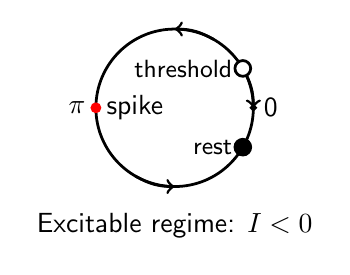
\begin{tikzpicture}
    \draw (0,0) circle [radius=1];
    \draw (0,-1.2) node[below]{Excitable regime: $I < 0$};
    \draw (-1,0) node[left]{$\pi$};
    \draw[fill=black, black] (1,0) circle [radius=0.025];
    \draw (1,0) node[right]{0};
    \draw[fill=red, red] (-1,0) circle [radius=0.05];
    \draw (-1,0) node[right]{spike};
    
    \draw[black, ->] (0.866, 0.5)to[out=-60,in=90](1,0);
    \draw[fill=white, draw=black] (0.866,0.5) circle [radius=0.1];
    \draw (0.866,0.5) node[left]{\small{threshold}};
    
    \draw[fill=black, draw=black] (0.866,-0.5) circle [radius=0.1];
    \draw (0.866,-0.5) node[left]{\small{rest}};
    
    \draw[black, ->] (0.5,0.866)to[out=150,in=0](0,1);
    \draw[black, ->] (-0.5,-0.866)to[out=-30,in=180](0,-1);
\end{tikzpicture}
\endminipage
\minipage{0.33\linewidth}
\centering
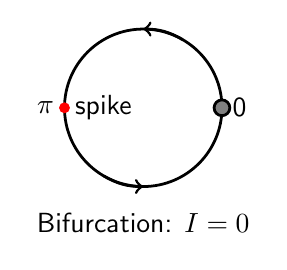
\begin{tikzpicture}
    \draw (0,0) circle [radius=1];
    \draw (0,-1.2) node[below]{Bifurcation: $I = 0$};
    \draw (1,0) node[right]{0};
    \draw[fill=red, red] (-1,0) circle [radius=0.05];
    \draw (-1,0) node[right]{spike};
    \draw (-1,0) node[left]{$\pi$};
    
    \draw[fill=gray, draw=black] (1,0) circle [radius=0.1];
    
    \draw[black, ->] (0.5,0.866)to[out=150,in=0](0,1);
    \draw[black, ->] (-0.5,-0.866)to[out=-30,in=180](0,-1);
\end{tikzpicture}
\endminipage
\minipage{0.33\linewidth}
\centering
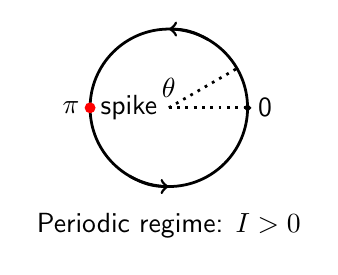
\begin{tikzpicture}
    \draw (0,0) circle [radius=1];
    \draw (0,-1.2) node[below]{Periodic regime: $I > 0$};
    \draw (-1,0) node[left]{$\pi$};
    \draw (1,0) node[right]{0};
    \draw[fill=black, black] (1,0) circle [radius=0.025];
    \draw[fill=red, red] (-1,0) circle [radius=0.05];
    \draw (-1,0) node[right]{spike};
    
    \draw[black, dotted] (0,0)to(1,0);
    \draw(0,0) node[above]{$\theta$};
    \draw[black, dotted] (0,0)to(0.866,0.5);
    
    \draw[black, ->] (0.5,0.866)to[out=150,in=0](0,1);
    \draw[black, ->] (-0.5,-0.866)to[out=-30,in=180](0,-1);
\end{tikzpicture}
\endminipage
\caption{SNIC bifurcation of the theta neuron model. A spike occurs when $\theta = \pi$. For $I < 0$, the neuron is in a rest state but \textsl{excitable}. For $I > 0$, $\dot{\theta} > 0$ so that $\theta$ moves continuously around the circle and we can observe \textsl{periodic} sustained spiking. The saddle-node bifurcation occurs at $I = 0$, so that $\theta$ will spike when it is larger than 0.}
\label{fig:thetaneuronbifurcationtikz}
\end{figure}

We can recognise the features of the class 1 model in Figure \ref{fig:ThetaNeuronResponseToCurrent}. This makes \eqref{eq:thetaneuron} the normal form of the \textit{saddle-node-on-invariant-circle} ($\SNIC$) bifurcation \cite{Luke2013}.

\begin{figure}[H]
\centering
\includegraphics[width = \textwidth]{../Figures/ThetaNeuronResponseToCurrent.pdf}
\caption{Properties of the theta neuron model, with solutions of \eqref{eq:thetaneuron} in blue, spikes marked in dotted lines, and the current $I$ in red. Left: the spike frequency of $\theta$ increases as $I$ is increased over time, which is the distinguishing feature of class 1 canonical models. Middle: spikes occur within a finite time period when $I > 0$ and within infite time when $I = 0$. Right: when $I$ is large, the neuron \textsl{bursts}.}
\label{fig:ThetaNeuronResponseToCurrent}
\end{figure}

Equilibria only exist for the \textsl{excitable} regime $I < 0$: 
\begin{align*}
\dot{\theta} &= 1-\cos \theta+I+I \cdot \cos \theta = (I+1)+(I-1) \cdot \cos \theta \\
\theta^{\ast}_{1, 2} &= \pm \arccos \left(\frac{I+1}{1-I}\right)+2 \pi n
\end{align*}
We can find the stability of the equilibria through:
\begin{align*}
\frac{\mathop{d}}{\mathop{d \theta}}((1-\cos \theta)+(1+\cos \theta) \cdot I) &= \sin \theta-\sin \theta \cdot I = (1-I) \cdot \sin \theta
\end{align*}
In the equilibria this yields:
\begin{align*}
\frac{\mathop{d}}{\mathop{d \theta}}\left( \theta^{\ast}_{1, 2} \right) &= \pm(1-I) \cdot \sqrt{1-\frac{I+1}{1-I}}=\pm(1-I) \cdot \frac{2 \sqrt{-I}}{1-I} = \pm2 \sqrt{-I}
\end{align*}
This yields a stable equilibrium point for $\theta^{\ast}_{1}$ and an unstable for $\theta^{\ast}_{2}$. This means that as $\theta$ gets perturbed above $\theta^{\ast}_{2}$, a spike occurs and $\theta$ converges to $\theta^{\ast}_{1}$. This is demonstrated in Figure \ref{fig:ThetaModelEquilibriumPoints}.
\begin{figure}[H]
\centering
\includegraphics[width = \textwidth]{../Figures/ThetaModelEquilibriumPoints.pdf}
\caption{Equilibria $\theta^{\ast}$ for different values of $I$. Left: $I = -1$ yields $\theta^{\ast}_{1,2} = \pm \frac{\pi}{2}$, one of the simulations is started exactly on the unstable equilibrium. Middle: $I = -0.5$. Right: bifurcation diagram of the \SNIC bifurcation, with the stable equilibria in blue, and the unstable in red.}
\label{fig:ThetaModelEquilibriumPoints}
\end{figure}


\subsection{Solutions for static currents} \label{sec:TheThetaNeuronModelSolutionPeriodics}
Gaining insight into \eqref{eq:thetaneuron} is hard, due to the difficulty of finding an analytical solution. However, it has been noted that there exists a simple transformation which yields (see \ref{app:TransformationToQIF}):
\begin{align}
V &\equiv \tan \left( \frac{\theta}{2} \right) \label{eq:QIFtransformation} \\
\dot{V} &= V^2 + I \label{eq:QIFmodel}
\end{align}
This model is called the \textsl{Quadratic Integrate and Fire model} (\QIF). \eqref{eq:QIFmodel} models the membrane potential of a neuron, which spikes to $=\infty$ when the neuron spikes and is reset at $-\infty$. The transformation \eqref{eq:QIFtransformation} is continuous between spikes, so insights from a solution for $V$ can be transformed directly. The equilibria of the \QIF model are simply $\pm \sqrt{I}$ so that we can express $\theta^{\ast}_{1, 2} = 2 \cdot\arctan \left( \mp \sqrt{I} \right)$ \cite{Gutkin2014}. \\

The solution for the excitable regime $I < 0$ is :
\begin{align}
V(t) = \frac{2 \sqrt{-I}}{1 - e^{2 t \sqrt{-I}}}-\sqrt{-I} \label{eq:ThetaNeuronModelSolutionPeriodicExcitable}
\end{align}
The solution at the bifurcation $I = 0$ is :
\begin{align}
V(t) = \frac{-1}{t} \label{eq:ThetaNeuronModelSolutionPeriodicBifurcation}
\end{align}
The solution for the periodic regime $I > 0$ is :
\begin{align}
V(t) = -\sqrt{I} \cdot \cot (t \sqrt{I}) \label{eq:ThetaNeuronModelSolutionPeriodic}
\end{align}
The solutions to \eqref{eq:ThetaNeuronModelSolutionPeriodicExcitable}-\eqref{eq:ThetaNeuronModelSolutionPeriodic} are described in \ref{app:ThetaModelSolutions}. Solutions for $\theta$ are found by taking the inverse of the transformation \eqref{eq:QIFtransformation}.

\subsection{Frequency response} \label{sec:TheThetaNeuronModelFrequencyResponse}
As we already saw in Figure \ref{fig:ThetaNeuronResponseToCurrent}, an increasing current increases the spiking frequency. We can compute this relationship by measuring how long it takes for $V$ to reach a spike: we solve \eqref{eq:ThetaNeuronModelSolutionPeriodic} for $t$ at $V(t) = +\infty$ in \ref{app:ThetaModelFrequencyResponse}. This yields the oscillation period $T = \frac{\pi}{\sqrt{I}}$ which we can see in Figure \ref{fig:ThetaNeuronResponseToCurrentPeriod}. 

We know that when $\theta > \theta^{\ast}_{2}$ a spike occurs. But the time that it takes to reach the spike can be arbitrarily long, depending on how far we are over $\theta^{\ast}_{2}$. So, spikes will occur, but after a delay that is dependant on the stimulus. Explicitly, if we perturb $\theta(0) = \theta^{\ast}_{2} + \varepsilon$ we obtain from  \cite{Gutkin2014}:
\begin{align*}
T_{\text {spike}} = \frac{-\tanh ^{-1}\left(1+\frac{\epsilon}{\sqrt{I}}\right)}{\sqrt{I}}
\end{align*}
The delay to the spike blows up as $\varepsilon \rightarrow$ 0 so that spikes may occur after a very large delay.

\begin{figure}[H]
\centering
\includegraphics[width = 0.75\textwidth]{../Figures/ThetaNeuronResponseToCurrentPeriod.pdf}
\caption{Frequency response of the theta model, with theoretical results in blue, and experimental results in black dots. For $I \leq 0$ the spike period is infinite, which is why we see the solutions to \eqref{eq:thetaneuron} approach $\theta = 0$ for $I = 0$.}
\label{fig:ThetaNeuronResponseToCurrentPeriod}
\end{figure}

In most of our future work, $I$ will not be a static current. We ask ourselves: how sensitively does $T$ depend on $I$ when $I$ is perturbed? We can measure this as a \textsl{relative} perturbation using $\mathop{dI}/I$ and $\mathop{dT/T}$ \cite{IntroductionModelingDynamics} :
\begin{align*}
\left| \frac{dT}{dI} \frac{I}{T} \right| &= \left| \frac{dT / T}{dI / I}\right| 
= \left|- \frac{\pi}{2} \left(\frac{1}{\sqrt{I}}\right)^3 \frac{I}{T} \right| 
= \left| \frac{\pi}{2} \left(\frac{T}{\pi}\right)^3 \frac{I}{T} \right| 
= \frac{1}{2} \left|\left(\frac{T}{\pi}\right)^2 \cdot \left(\frac{\pi}{T}\right)^2 \right| = \frac{1}{2}
\end{align*}
Hence, a 1\% change in $I$ will result in a 0.5 \% change in the period.


\subsection{Phase response} \label{sec:TheThetaNeuronModelPhaseResponse}
Perturbations on the period can also be understood from the perspective of the phase. Changes to the phase $\theta$ can delay or advance the event of a spike, and in general this depends on exactly when the stimulus occurs. The phase response curve (\PRC) gives us exactly that relation \cite{Perez2020, Gutkin2014}.

For infinitesimally small perturbations to the phase, we can find the \PRC as the \textsl{adjoint} of the solution as:
\begin{align*}
\PRC(t)=\frac{1}{d V / d t}=\frac{1}{2 \sqrt{I}}(1-\cos (2 \cdot t \cdot \sqrt{I}))
\end{align*}


\subsection{Networks of theta neurons}
We can easily extend the model to networks of neurons:
\begin{align}
\dot{\theta}_{i} &=\left(1-\cos \theta_{i}\right)+\left(1+\cos \theta_{i}\right) \cdot \left[\eta_{i} + \kappa \cdot I_{i}(t)\right] \qquad \theta_i \in \T^N  \label{eq:thetaneuronnetwork} \\
I_{i}(t) &=\frac{1}{\kmean} \sum_{j=1}^{N} A_{i j} \cdot \mathcal{P}_{n}(\theta_{j}) \label{eq:thetaneuronnetworkcurrent}
\end{align}
where the excitability $\eta_i$ is drawn from a distribution $g(\eta \rvert \eta_0, \sigma)$ and $\mathcal{P}(\theta)  = a_n(1 - \cos \theta)^n$ models synaptic coupling by a pulse-shaped signal, emitted when a neuron fires. $n$ models the sharpness of the pulse, and $a_n$ is a normalisation constant. We will take $n=2$ from here in as in\cite{Luke2013}, \cite{OttAntonsen2017}, \cite{Martens2020}. 


Another type of coupling is proportional to the difference in voltage between neurons \cite{Martens2020}. Note that for a fully connected network, \eqref{eq:thetaneuronnetworkcurrent} reduces to the scenarios in \cite{Luke2013} and \cite{Martens2020}.

In \eqref{eq:thetaneuronnetwork} we see everything come together: changes to the phase $\theta_i$ come from $\dtheta_i$, which in turn depends on $I$, which depends on all phases in the network.




% !TEX root = ../main.tex
\newpage
\section{Network Topologies} \label{NetworkTopologies}


\subsection{Fixed-degree networks}
\noindent A network consists of nodes, connected by links. The most simple network is one where all the nodes are connected, and so all nodes have a degree of $N$. In general, we can make networks where all nodes have the same degree $k = \kmean$:
\begin{align}
P(k) = \left\{\begin{array}{ll}\kmean & \text{if } k=\kmean \\0 & \text{otherwise}\end{array}\right. \label{eq:diracpdf}
\end{align}
We will refer to these networks as fixed-degree networks.


\subsection{Random / Erd{\"o}s-R{\'e}ny networks}
In 1959 Erd{\"o}s and R{\'e}ny published their work on random graphs\cite{RandomGraphs1959}, where links are established if a random uniformly distributed number is higher than a threshold $p$. The degrees follow a binomial distribution: 
\begin{align}
P(k)=\left(\begin{array}{c}N-1 \\ k\end{array}\right) p^{k}(1-p)^{N-1-k} \label{eq:binomialpdf}
\end{align}
with a mean $\mu = p(N-1)$ and standard deviation $\sigma = \mu(1-p)$. For networks where $\kmean \ll N$, the network can be well approximated by a Poisson distribution:
\begin{align}
P(k) = e^{-\kmean} \frac{\kmean^{k}}{k !} \label{eq:poissonpdf}
\end{align}
with a mean $\mu = \kmean$ and standard deviation $\sigma = \sqrt{\kmean}$. Both \eqref{eq:binomialpdf} and \eqref{eq:poissonpdf} describe similar quantities, but the latter is used more often due to its analytical simplicity \cite{BarabasiNetworkBook2016}.


\subsection{Scale-free networks}
What we can often observe in nature is the preferential attachment to nodes with a high degree \cite{Bullmore2010}: the rich or famous tend to get more rich or famous. This trait is also described as the 80/20 rule by Pareto. Networks with this property consist of a small number of highly connected nodes, and a large number of low degree nodes. We can represent this with a power law distribution:
\begin{align}
P(k) = A k^{-\gamma} \label{eq:scalefreepdf}
\end{align}
with $A$ is a constant so that $\sum_{k=1}^{\infty} P(k) = 1$. We can also see that $A \sum_{k=1}^{\infty} k^{-\gamma} = 1$ so that $A = \sum_{k=1}^{\infty} k^{\gamma} = 1/\zeta(k)$, the Riemann Z{\'e}ta function \cite{BarabasiNetworkBook2016}. 

Networks with a distribution like \eqref{eq:scalefreepdf} are called \textit{scale-free} networks, as they lack an internal scale to represent the magnitude of the network: we can observe \eqref{eq:scalefreepdf} on different scales like the probability of two Hollywood actors appearing in a movie, or the connections between web pages on the internet \cite{Barabasi2003}. One description that comes close is the \textit{natural cutoff} $k_{\text{max}}$, the expected degree of the largest degree in the network. As we only expect the largest hub to be the only hub in the domain $[k_{\text{max}}, +\infty]$:
\begin{align*}
\int_{k_{\text{max}}}^{\infty} P(k) dk=\frac{1}{N}
\end{align*}
For \eqref{eq:scalefreepdf} this results in:
\begin{align}
k_{\text{max}}=k_{\text{min}} \cdot N^{\frac{1}{\gamma-1}} \label{eq:scalefreecutoff}
\end{align}
which shows that there might be large differences in size between the nodes. There are constraints on $\gamma$ to yield a scale-free network. When $0 < \gamma < 2$ the largest hub grows faster than $N$, so once its degree exceeds $N-1$ there are no more new nodes to connect to. A rigorous proof is given in \cite{Bassler2011}. For $\gamma = 2$, the system grows linearly, as we can see in \eqref{eq:scalefreecutoff}. When $2 < \gamma \leq 3$ we find the most scale-free networks, as for $\gamma > 3$ hubs are not sufficiently large and numerous to have much influence on the network
\cite{BarabasiNetworkBook2016}.

% !TEX root = ../main.tex
\newpage
\section{Mean Field Reductions}
\subsection{The Ott-Antonsen manifold for fully connected networks}
In \cite{OttAntonsen2008, OttAntonsen2009, OttAntonsen2010} a method was published to predict the dynamics of the order parameter \eqref{eq:orderparameter}. The exact \textsl{mean-field reduction} (\MFR) yields exact solutions to 

\subsection{Dynamics of the mean field}

\subsection{The Ott-Antonsen extension to arbitrary network topologies}
In \cite{OttAntonsen2017} the authors extended their work to include networks with arbitrary degree distributions.
% !TEX root = ../main.tex
\newpage
\section{\mywork Mean Field Reductions for undirected graphs}
\subsection{Directed graphs as permutations}
So how can we use the \MFR efficiently when the network is a directed graph with an asymmetrical adjacency matrix? Let's investigate.
\begin{itemize}
\item Sampling $\kinb$ and $\koutb$ from a bivariate distribution requires us to find the marginal distribution of $P$ for $\kinb$, sampling $\kinbi$, and then sampling $\koutbj$ from $P$ while keeping $\kinbi$ fixed. This is a cumbersome process. And what relation would there be between $\kinb$ and $\koutb$?
\item However, if we assume that the marginal distributions for $\kinb$ an $\koutb$ are independent, there is a simplification to be found. We can even assume that the two marginal distributions are identical univariate distributions. 
\item Hence, we can sample $\kinb$ from a univariate distribution and find $\koutb = \permute ( \kinb )$ so that the total number of links remains constant. 
\end{itemize}

This hypothesis can be tested: we assume that $P(\k) = P(\kin) \cdot P(\kout)$ so that $P$ consists of two identical and independent distributions, given by the distributions presented in Chapter \ref{sec:NetworkTopologies}. Then, we sample $\kinb \sim P(\kin)$ and perform a permutation to find all node degrees $\k_j$. The surface given by $P$ and the histogram of $\k_j$ have been plotted in Figure \ref{fig:2Ddistributions}. As we can see, the variates follow the distribution well. 

\begin{figure}[H]
\centering
\includegraphics[trim=2.5cm 0cm 2.5cm 0cm, clip=true, width = \textwidth]{../Figures/Distributions/2D.png}
\caption{Bivariate distributions for different network topologies, using 10$^4$ number of samples. The surface given by $P(\k)$ is well approximated by the histogram of variates sampled from a univariate distribution. $\kmean =  2 \times 10^3$ for all topologies, $p \approx 0.2$ for the random network and $\gamma = 4.3$ for the scale-free network.}
\label{fig:2Ddistributions}
\end{figure}


\subsection{Building the adjacency matrix} \label{sec:buildingA}
If we want to simulate the network of theta neurons \eqref{eq:thetaneuronnetworkcurrent} we need to construct the adjacency matrix. We can find an exact solution for $A$ given the degree vectors in \eqref{eq:definekinkoutfromP}. $A_{ij}$ represents a directed graph, but $A_{ij} \neq A_{ji}$ is not a necessary condition. For the elements of $A_{ij}$ we need to find $N^2$ number of variables. We have the following constraints:
\begin{enumerate}
\item The column- and row-sums of $A_{ij}$ must be equal to $\kinb$ and $\koutb$, see \eqref{eq:definekinkoutfromA}. 2$N$ constraints.
\item Self-coupling is mandatory: $A_{ii} = \boldsymbol{1}$. $N$ constraints.
\item The total number of links is constant: $\sum_{i=1}^{N} \kinbi \equiv \sum_{j=1}^{N} \koutbj \equiv \sum_{i,j=1}^{N}A_{i j}$. 1 constraint.
\end{enumerate}
This means that there are $N^2 - (3N + 1)$ variables to find. Once a solution has been found, $A_{ij}$ can be switched with element $A_{ic}$ if $A_{ij} \neq A_{ic}$ and $A_{rj}$ with $A_{rc}$, which yields a new feasible solution. The number of switches one can make is high, and therefore we can simply try a stochastic approach to obtain $A$:
\begin{enumerate}
\item Choose a random row $i \in [1,N]$. $A_{i,i} = 1$, so we need $m = \kinbi - 1$ elements that are 1.
\item Perform $\permute ( \koutbj, j \neq i)$ and therein find the indices $\boldsymbol{\ell}$ of the $m$ first largest elements. 
\item Set $A_{il} = 1 \: \: \forall \: \: l \in \permuteinv (\boldsymbol{\ell})$.
\end{enumerate}
Algorithms that find the largest value in a vector start from the first or the last element. The permutation allows us to find different maxima every time by shuffling the vector.

\begin{figure}[H]
\centering
\begin{subfigure}[b]{0.32\linewidth}
   \centering
  \includegraphics[width=\linewidth, trim={0.5cm 0.5cm 1cm 0.5cm },clip]{../Figures/Adjacency matrices/A_fixeddegree.pdf}
%   \caption{Adjacency matrix for a fixed-degree network.}
 %  \label{fig:A_fixeddegree} 
\end{subfigure} \hfill
\begin{subfigure}[b]{0.32\linewidth}
   \centering
  \includegraphics[width=\linewidth, trim={0.5cm 0.5cm 1cm 0.5cm },clip]{../Figures/Adjacency matrices/A_random.pdf}
%   \caption{Adjacency matrix for a fixed-degree network.}
%   \label{fig:MFRPSS}
\end{subfigure} \hfill
\begin{subfigure}[b]{0.32\linewidth}
   \centering
  \includegraphics[width=\linewidth, trim={0.5cm 0.5cm 1cm 0.5cm },clip]{../Figures/Adjacency matrices/A_scalefree.pdf}
%   \caption{Adjacency matrix for a fixed-degree network.}
%   \label{fig:MFRCPW}
\end{subfigure}
   \caption{Adjacency matrices for different types of networks with $N$ = 500 and $\kmean$ = 100. We can see how the fixed-degree network is quite homogeneous, while the random network shows some more clustering. The scale-free network has a low number of nodes with a very high degree, which is why we see vertical and horizontal stripes in the adjacency matrix.}
   \label{fig:adjacencymatrices}
\end{figure}


\subsection{Fixed-degree networks as a baseline}
\begin{figure}[H]
\centering
\includegraphics[width = \textwidth]{../Figures/InspectMeanFieldFixedDegree.pdf}
\caption{Comparison}
\label{fig:InspectMeanFieldFixedDegree}
\end{figure}

% !TEX root = ../main.tex
\newpage
\section{Hebbian Learning and Synaptic Plasticity}


\subsection{What does it mean to learn?}
Lorem ipsum dolor sit amet, consectetur adipiscing elit. Quisque nisl eros, 
pulvinar facilisis justo mollis, auctor consequat urna. Morbi a bibendum metus. 
Donec scelerisque sollicitudin enim eu venenatis. Duis tincidunt laoreet ex, 
in pretium orci vestibulum eget.


\subsection{Hebbian Learning}
Lorem ipsum dolor sit amet, consectetur adipiscing elit. Quisque nisl eros, 
pulvinar facilisis justo mollis, auctor consequat urna. Morbi a bibendum metus. 
Donec scelerisque sollicitudin enim eu venenatis. Duis tincidunt laoreet ex, 
in pretium orci vestibulum eget.


\subsection{Anti-hebbian learning}
Lorem ipsum dolor sit amet, consectetur adipiscing elit. Quisque nisl eros, 
pulvinar facilisis justo mollis, auctor consequat urna. Morbi a bibendum metus. 
Donec scelerisque sollicitudin enim eu venenatis. Duis tincidunt laoreet ex, 
in pretium orci vestibulum eget.


\subsection{Spike-timing dependant plasticity}
Lorem ipsum dolor sit amet, consectetur adipiscing elit. Quisque nisl eros, 
pulvinar facilisis justo mollis, auctor consequat urna. Morbi a bibendum metus. 
Donec scelerisque sollicitudin enim eu venenatis. Duis tincidunt laoreet ex, 
in pretium orci vestibulum eget.


\subsection{Intrinsic plasticity}
Lorem ipsum dolor sit amet, consectetur adipiscing elit. Quisque nisl eros, 
pulvinar facilisis justo mollis, auctor consequat urna. Morbi a bibendum metus. 
Donec scelerisque sollicitudin enim eu venenatis. Duis tincidunt laoreet ex, 
in pretium orci vestibulum eget.

% !TEX root = ../main.tex
\newpage
\section{\mywork Emerging Network Topologies}
\subsection{\STDP applied to networks of theta neurons}
\textcolor{red}{TODO}: \textsl{explain in detail how the different methods \cref{eq:KempterSTDPFormulation2,eq:SongSTDPFormulation} will be implemented, using \STDP coupled with \IP.}


\subsection{Results}
\textcolor{red}{TODO}: \textsl{describe the emergent behaviour.}


% !TEX root = ../main.tex
\newpage
\section{Conclusion and Discussion} \label{sec:ConclusionAndDiscussion}
%\textcolor{red}{TODO}: \textsl{what did we achieve with this work?}

Starting from the Theta neuron model, we have holistically discussed its use in directed networks and described synchronisation of different network topologies, simplifying the analysis with the \MFR. We have proven that from random initial topological conditions, a regular network structure can appear. Obtaining these results is the first step towards a unification in the theory of the dynamics \textsl{on} and \textsl{of} networks. \\

Even though both fields have been well-established, currently there exists no theory that takes both approaches into account. The science of the different fields is scattered, a schism that is represented by the structure of this report. The only constant is the description of the behaviour of networks, which was rigorously adapted for this work. Going forward, it would be interesting to see whether a similar approach as in the \MFR can be taken: if the network dynamics can be represented per node degree, then why not find a learning strategy that allows for a coupling matrix defined on $\mathbb{N}^{N \times N}$? Or can we perhaps bin the node degrees so that even less equations are necessary for the \MFR to function? \\

These questions are the seed for a future investigation.


\subsection{Further investigation of initial and final conditions}
The initial conditions of the different systems obtained in Chapter \ref{sec:initialconditions} by numerically solving for $f(z) = \| Z(0) - \bar{Z}(0) \|$ are satisfactory, but can be improved upon. The distribution of degrees over the attractive manifold can be taken into account by further analysis on the final conditions, and we should obtain a better understanding of the location of the manifold with respect to the resulting point in $\bar{Z}$. Then, a second condition can be added so that the numerical solution of $f$ converges to the manifold. 

In the current implementation, there is no objective function for the optimisation. $f$ is solved as an equality constraint so that the solution is exact and not just a minimum, and the constraint $| z | \leq 1$ is solved as an inequality. This leaves the objective function free to take the manifold into account: a metric like the Kullback-Leibler divergence can be introduced to take the target distribution into account. 


\subsection{A learning strategy with desirable properties}
In Chapter \ref{sec:HebbianLearningAndSynapticPlasticity}, two different learning strategies were presented, and in Chapter \ref{sec:EmergingNetworkTopologies} their functionality was discussed. The feedback loops between $W$ and $\Delta K$ make it hard to find a formulation that would guarantee a stable network topology, without the artificial bounds on $K$. Another challenge is allowing inhibitive \textsl{and} excitatory coupling, which no other work has touched upon.

A constant in the formulation of a learning strategy is the in- and outgoing spike trains: 
\begin{align}
\Delta K_{ij} \sim \sum_{t_{j}^{f}, \: t_i^{n} \in \mathcal{T}} \hspace{-2mm} W (t_{j}^{f}-t_i^{n} )
\end{align}
We can then easily punish nodes with large degrees by postulating:
\begin{align}
\Delta K_{ij} \sim - (K_{ij}) \circ \rvert K_{ij} \rvert
\end{align}
The Hadamard product $\circ$ ensures that the sign of the coupling strength is preserved, so that the restraint to halt the continuous potentiation works symmetrically, inspired by Oja's rule\cite{ChrolCannon2014}. We might also direct nodes with a low degree towards zero, or stimulate them to grow. The options explored by the machine learning community can be an inspiration for future research.


\subsection{Symmetry of the learned degree distributions}
The degree distributions resulting from the learning procedure in Chapters \ref{sec:STDPlearning} and \ref{sec:STDPandIPlearning} should be investigated further, as it appears that $\kinb$ and $\koutb$ are variates from the same univariate distribution. The impact of using a bimodal degree distribution, which was the result of using $W_C$, is currently unknown.

Perhaps the differences we observed between the \MFR and the solutions of the whole network in Chapter \ref{sec:resArbNetw} can be explained by the fact that fixed-degree and random networks have a degree distribution with $\kmean$ as the axis of symmetry, which the scale-free distribution does not have. The latter showed large differences between the two approaches.


\subsection{Synchronisation and spiking rate}
In accordance with most of the work conducted on the \MFR, the order parameter was used to measure synchrony in the network. In the context of \STDP and \IP, a better metric could have been the mean firing rate, the average neural activity of a node in the past:
\begin{align}
\rho(t)=\frac{1}{N} \sum_{j=1}^{N} \sum_{n} \delta\left(t-t_{j}^{n}\right)
\end{align}
The mean firing rate is related to the order parameter through:
\begin{align}
\rho(t) = \frac{1}{\pi} \Re \left(\frac{1-Z(t)^c}{1+Z(t)^c}\right)
\end{align}
In \cite{Montbrio2015}, a firing rate \MFR for networks of the Theta model was proposed, yielding a different light on the firing dynamics. This metric could easily be introduced in the analysis of the \MFR in Chapter \ref{sec:MFRSUndirected} and the learning procedures in Chapter \ref{sec:EmergingNetworkTopologies}.






\newpage
\bibliographystyle{utphys}
\small{\bibliography{references}}

% !TEX root = ../main.tex

\newpage
\appendix
\section{Appendix} \label{sec:Appendix}

\subsection{Transformation to the QIF model} \label{app:TransformationToQIF}
We prove that the transformation \eqref{eq:QIFtransformation} holds from the \QIF model \eqref{eq:QIFmodel} to the Theta model \eqref{eq:thetaneuron}.
\begin{align*}
V &\equiv \tan \left( \frac{\theta}{2} \right) \quad \longrightarrow \quad
\frac{\mathop{d V}}{\mathop{d t}} = \frac{1}{2 \cos ^{2}\left(\frac{\theta}{2}\right)} \frac{d \theta}{ \mathop{d t}}
\end{align*}
Insert into $\frac{\mathop{d V}}{\mathop{d t}}= V^2 + I$:
\begin{align*}
\frac{\mathop{d \theta}}{\mathop{d t}} &= 2\left(\cos ^{2}\left(\frac{\theta}{2}\right) \cdot \tan ^{2}\left(\frac{\theta}{2}\right)+\cos ^{2}\left(\frac{\theta}{2}\right) \cdot I \right) = 2\left(\sin ^{2}\left(\frac{\theta}{2}\right)+\cos ^{2}\left(\frac{\theta}{2}\right) \cdot I \right)
\end{align*}
Using $\cos ^{2}\left(\frac{\theta}{2}\right) = \frac{1+\cos \left(\frac{\theta}{2}\right)}{2}$ and $\sin ^{2}\left(\frac{\theta}{2}\right)=\frac{1-\cos \left(\frac{\theta}{2}\right)}{2}$:
\begin{align*}
\dot{\theta} &=2\left(\frac{1-\cos \theta}{2}+\left(\frac{1+\cos \theta}{2}\right) \cdot I \right) =(1-\cos \theta)+(1+\cos \theta) \cdot I
\end{align*}
This proves that the transformation is correct.

 
\subsection{Solutions to the QIF model} \label{app:ThetaModelSolutions}
Depending on the value of $I$, we can distinguish multiple solutions  \cite{Perez2020}. In all cases we can integrate through the separation of variables. Solutions are bound to start at $V(0)$ after a spike has occured. Solutions for $\theta$ are found by taking the inverse of the transformation \eqref{eq:QIFtransformation}.

\subsubsection{Solving for \texorpdfstring{$I = 0$}{TEXT}}
\begin{align*}
\int_{V(0)}^{V(t)} \frac{\mathop{dv}}{v^2} &= \frac{1}{v}\Big\rvert_{V(0)}^{V(t)} = - \frac{1}{V(t)} + \frac{1}{V(0)} = \int_0^t \mathop{d\tau} = t \\
V(t) &= \lim_{V(0) \rightarrow - \infty} \frac{V(0)}{1-V(0)t} \underset{\frac{\infty}{\infty}}{\overset{\mathrm{H}}{=}} \frac{-1}{t}
\end{align*}


\subsubsection{Solving for \texorpdfstring{$I > 0$}{TEXT}}
%Separate the variables as $\frac{\mathop{dv}}{v^2 + I} = \mathop{dt}$ and integrate from $t=0$:
\begin{align*}
\int_{V(0)}^{V(t)} \frac{\mathop{dv}}{v^2 + I} &= \int_{V(0)}^{V(t)} \frac{I}{\left(\frac{v}{\sqrt{I}}\right)^2 + 1} \mathop{dv}
\quad \longrightarrow \quad x = \frac{v}{\sqrt{I}} \quad \mathop{dx} = \frac{\mathop{dv}}{\sqrt{I}} \\
&= \int_{\frac{V(0)}{\sqrt{I}}}^{\frac{V(t)}{\sqrt{I}}} \frac{I}{x^2 + 1} \mathop{dx}= \frac{1}{\sqrt{I}} \arctan(x) \Big \rvert_{\frac{V(0)}{\sqrt{I}}}^{\frac{V(t)}{\sqrt{I}}} 
= \frac{1}{\sqrt{I}} \left( \arctan \left( \frac{V(t)}{\sqrt{I}} \right) - \arctan \left( \frac{V(0)}{\sqrt{I}} \right) \right)\\
\int_0^t \mathop{d\tau} &= t \\
V(t) &= \lim_{V(0) = -\infty} \sqrt{I} \cdot \tan \left( t \sqrt{I} + \arctan \left( \frac{V(0)}{\sqrt{I}} \right) \right) = \sqrt{I} \cdot \tan \left( t \sqrt{I} - \frac{\pi}{2} \right) \\
&=  \sqrt{I} \cdot \cot \left( t \sqrt{I} \right) 
\end{align*}

\subsubsection{Solving for \texorpdfstring{$I < 0$}{TEXT}}
%Change variables: $I = -\tilde{I}^2$. Separate variables as $\frac{\mathop{dv}}{v^2 - \tilde{I}^2} = \mathop{dt}$ and integrate from $t = 0$:
\begin{align*}
\int_{V(0)}^{V(t)} \frac{\mathop{dv}}{v^2 - \tilde{I}^2} &= \int_{V(0)}^{V(t)} \frac{\mathop{dv}}{(v+\tilde{I})(v-\tilde{I})} 
= \frac{1}{2 \tilde{I}} \int_{V(0)}^{V(t)} \frac{\mathop{dv}}{v-\tilde{I}}-\frac{1}{2 \tilde{I}} \int_{V(0)}^{V(t)} \frac{\mathop{dv}}{v+\tilde{I}} \\
%&= \frac{1}{2 \tilde{I}} \log (v-\tilde{I}) -\frac{1}{2 \tilde{I}} \log (v+\tilde{I})\Big \rvert_{V(0)}^{V(t)} 
&= \frac{1}{2 \tilde{I}} \log \left(1-\frac{2 \tilde{I}}{v+\tilde{I}}\right) \Big \rvert_{V(0)}^{V(t)} 
= \int_0^t \mathop{d\tau} = t \\
V(t) &= \lim_{V(0) = -\infty} \frac{2 \sqrt{-I}}{1 - \left(1-\frac{2 \sqrt{-I}}{V(0)+\sqrt{-I}}\right)\cdot e^{2 t \sqrt{-I}}}-\sqrt{-I}\\
&= \frac{2 \sqrt{-I}}{1 - e^{2 t \sqrt{-I}}}-\sqrt{-I}
\end{align*}


\subsection{Frequency response of the neuron models} \label{app:ThetaModelFrequencyResponse}
We perform an integration vrom
\begin{align*}
T = \int_{V(0)}^{+\infty} \frac{\iota}{\left(\frac{v}{\sqrt{\iota}}\right)^2 + 1} dv 
\underset{x = \frac{v}{\sqrt{\iota}} \: \:dx = \frac{dv}{\sqrt{\iota}}}{=} 
\int_{\frac{V(0)}{\sqrt{\iota}}}^{+\infty} \frac{\iota}{x^2 + 1} dx 
= \frac{1}{\sqrt{\iota}} \arctan(x) \rvert_{\frac{V(0)}{\sqrt{\iota}}}^{+\infty} 
= \frac{1}{\sqrt{\iota}} \left( \frac{\pi}{2} - \arctan \left( \frac{V(0)}{\sqrt{\iota}} \right) \right)
\end{align*}

If then $V(0) = –\infty$ the time between spikes is:

\begin{align*}
T = \lim_{V(0) \rightarrow -\infty} \frac{1}{\sqrt{\iota}} \left( \frac{\pi}{2} - \arctan \left( \frac{V(0)}{\sqrt{\iota}} \right) \right) = \frac{1}{\sqrt{\iota}} \left( \frac{\pi}{2} - \left( - \frac{\pi}{2} \right) \right)
= \frac{\pi}{\sqrt{\iota}}
\end{align*}

So the frequency of oscillation is proportional to $\sqrt{\iota}$. This result is valid for the theta and QIF models.


\subsection{Jacobian of the Ott-Antonsen manifold}
\subsection{Jacobian of the Ott-Antonsen extended manifold}









\end{document}
